\begin{frame}{Example: The UCI Wine Dataset}

    \begin{columns}
        \begin{column}{0.51\linewidth}
    \begin{itemize}
        \setlength\itemsep{1em}
        \item Identify an Italian wine variety based on its color intensity and proline content.
        \item 177 data points $(x_{i,0}, x_{i,1}, y_i)$
    \end{itemize}
        \end{column}
        \begin{column}{0.5\linewidth}
            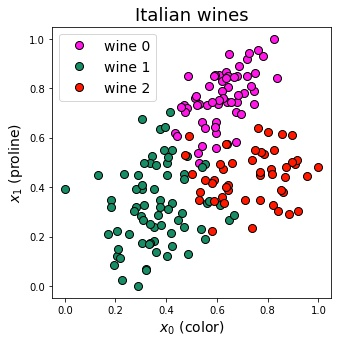
\includegraphics[scale=0.45]{wines.jpg}
        \end{column}
    \end{columns}

\end{frame}

\begin{frame}
    \frametitle{ML model 1: nearest neighbor classifier}
\begin{columns}
    \begin{column}{0.5\linewidth}
    \[
        f(x) = y_{I(x)},
    \]
    where
    \[
        I(x) = \argmin_i \|x_i-x\|
    \]
    \end{column}
    \begin{column}{0.5\linewidth}
        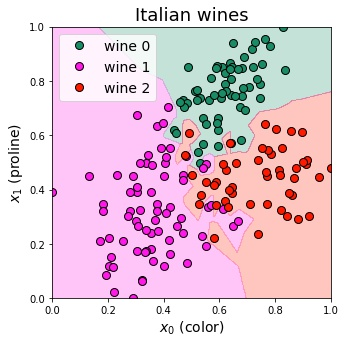
\includegraphics[scale=0.45]{wines-nn.jpg}
    \end{column}
\end{columns}
\end{frame}

\begin{frame}
    \frametitle{ML model 2: decision tree classifier}

    \begin{textblock*}{0in}(0.08in,1in) % {block width} (coords)
        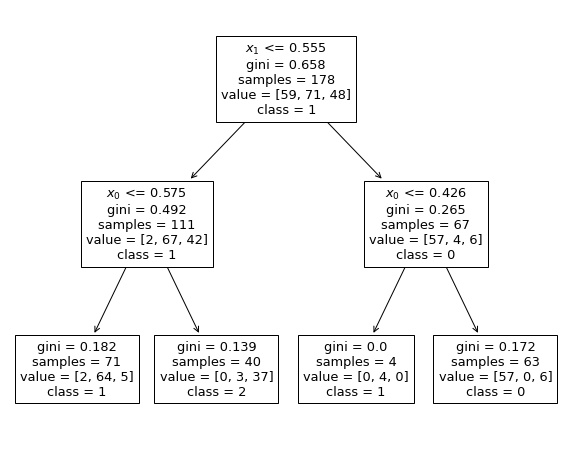
\includegraphics[scale=0.4]{wines-dt-tree.jpg}
    \end{textblock*}
    \begin{textblock*}{0in}(2.8in,0.3in) % {block width} (coords)
        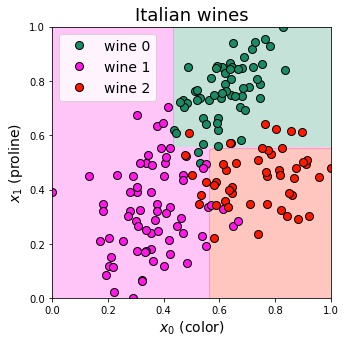
\includegraphics[scale=0.45]{wines-dt.jpg}
        \end{textblock*}
\end{frame}

\begin{frame}
    \frametitle{ML model 3: logistic regression}

    \begin{columns}
        \begin{column}{0.5\linewidth}
        \begin{align*}
            f(x) &= \argmax p(x),\\
            \intertext{where}
            p(x) &= \begin{bmatrix}
                p_0(x)\\ p_1(x)\\p_2(x)
            \end{bmatrix}\\
            &= \softmax(Wx + b)
        \end{align*}

        The parameters $W$ and $b$ are learned from data.
        \end{column}
        \begin{column}{0.5\linewidth}
            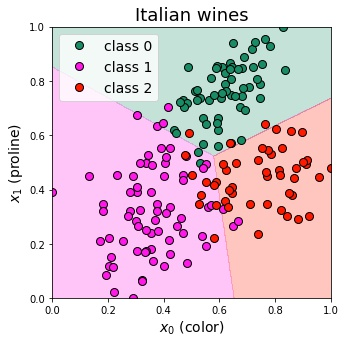
\includegraphics[scale=0.45]{wines-lr.jpg}
        \end{column}
    \end{columns}
\end{frame}
